\chapter{El corazón y la sangre}\label{ch:g4:heart-and-blood}

Apoya dos dedos --- no el pulgar --- en la cara interna de la \omterm{def:g1:my-body:joint}{muñeca},
debajo de la base del pulgar, y espera. Ahí está: un golpecito
pequeño y constante, una y otra vez, más o menos una vez por segundo.
Ese golpecito es tu \omterm{def:g4:heart-and-blood:heart}{corazón} trabajando, notado desde lejos. Late desde
antes de que nacieras y es el motor del servicio de reparto del cuerpo.

\section{La sangre, el servicio de reparto del cuerpo}

\begin{proposition}[Lo que transporta la sangre]\label{prop:g4:heart-and-blood:carries}
La \emph{sangre}\index{sangre} es un líquido que llega a todos los
rincones del cuerpo, y es el transportista del cuerpo:
\begin{itemize}
  \item en el \omterm{def:g4:journey-of-food:tract}{intestino delgado} recoge los \emph{\omterm{def:g4:journey-of-food:digestion}{nutrientes}}
        (\cref{prop:g4:journey-of-food:absorb});
  \item en los \omterm{def:g4:breathing:organs}{pulmones} recoge el \emph{oxígeno}
        (\cref{prop:g4:breathing:exchange});
  \item los reparte a todas las partes del cuerpo --- \omterm{def:g3:bones-and-muscles:muscle}{músculos},
        cerebro, \omterm{def:g3:bones-and-muscles:skeleton}{huesos}, \omterm{def:g1:the-five-senses:sense}{piel};
  \item a la vuelta se lleva los desechos y entrega el dióxido de
        carbono a los \omterm{def:g4:breathing:organs}{pulmones} para que se espire.
\end{itemize}
\end{proposition}
\admitted

\begin{example}[Una ronda de reparto]\label{ex:g4:heart-and-blood:round}
Sigue una gota de \omterm{prop:g4:journey-of-food:absorb}{sangre}: al pasar por los \omterm{def:g4:breathing:organs}{pulmones} se vuelve roja
brillante, cargada de oxígeno; el \omterm{def:g4:heart-and-blood:heart}{corazón} la manda fuera; en el
\omterm{def:g3:bones-and-muscles:muscle}{músculo} de una \omterm{def:g1:my-body:parts}{pierna} que corre entrega el oxígeno y los \omterm{def:g4:journey-of-food:digestion}{nutrientes},
carga dióxido de carbono y se oscurece; de vuelta en el \omterm{def:g4:heart-and-blood:heart}{corazón}, la
mandan a los \omterm{def:g4:breathing:organs}{pulmones} a descargar y a recargar --- y otra vez fuera.
Una ronda completa dura bastante menos de un minuto.
\end{example}

\begin{definition}[Vasos sanguíneos]\label{def:g4:heart-and-blood:vessels}
La \omterm{prop:g4:journey-of-food:absorb}{sangre} viaja por unos tubos llamados \emph{vasos
sanguíneos}\index{vaso sanguíneo}: anchos al salir del \omterm{def:g4:heart-and-blood:heart}{corazón} y al
entrar en él, y que se ramifican cada vez más finos --- hasta vasos
del grosor de un cabello que se cuelan entre las partes del cuerpo, donde
se entregan los repartos. Puestos uno detrás de otro, los vasos de un
cuerpo alcanzarían decenas de miles de kilómetros.
\end{definition}

\begin{remark}[Ver los vasos]\label{rem:g4:heart-and-blood:see}
Mírate la cara interna de la \omterm{def:g1:my-body:joint}{muñeca}: líneas azuladas bajo la \omterm{def:g1:the-five-senses:sense}{piel} ---
\omterm{def:g4:heart-and-blood:vessels}{vasos sanguíneos} camino del \omterm{def:g4:heart-and-blood:heart}{corazón}. Una \omterm{def:g1:my-body:joint}{rodilla} raspada enseña el
otro extremo de la red: hasta el corte más fino encuentra \omterm{prop:g4:journey-of-food:absorb}{sangre},
porque los \omterm{def:g4:heart-and-blood:vessels}{vasos} más finos están en todas partes.
\end{remark}

\section{El corazón, la bomba}

\begin{definition}[El corazón]\label{def:g4:heart-and-blood:heart}
El \emph{corazón}\index{corazón} es un \omterm{def:g3:bones-and-muscles:muscle}{músculo} hueco, más o menos del
tamaño del puño de su dueño, en el centro del pecho detrás de la caja
torácica. Al apretar --- un \emph{latido}\index{latido} --- empuja la
\omterm{prop:g4:journey-of-food:absorb}{sangre} por los \omterm{def:g4:heart-and-blood:vessels}{vasos}. Tiene dos lados: el lado derecho bombea \omterm{prop:g4:journey-of-food:absorb}{sangre} a
los \emph{\omterm{def:g4:breathing:organs}{pulmones}} para cargar oxígeno; el lado izquierdo bombea la
\omterm{prop:g4:journey-of-food:absorb}{sangre} rica en oxígeno a \emph{todo el cuerpo}.
\end{definition}

\begin{omfigure}
\begin{tikzpicture}[scale=0.95]
  % heart: two chambers schematic
  \draw[thick, fill=omThm!10] (0,0)
    .. controls (-1.5,0.9) and (-1.3,2.3) .. (-0.35,2.3)
    .. controls (-0.05,2.3) and (0.0,2.15) .. (0.0,2.05)
    .. controls (0.0,2.15) and (0.05,2.3) .. (0.35,2.3)
    .. controls (1.3,2.3) and (1.5,0.9) .. (0,0);
  \draw[thick] (0,2.05) -- (0,0.35);
  \node[font=\small, align=center] at (-0.55,1.45) {lado\\ derecho};
  \node[font=\small, align=center] at (0.55,1.45) {lado\\ izquierdo};
  % arrows: right side to lungs
  \draw[->, very thick, omDef] (-0.55,2.3) .. controls (-0.8,3.0)
    .. (-1.9,3.2)
    node[left, font=\small, omDef, align=center] {a los pulmones:\\ cargar oxígeno};
  \draw[->, very thick, omDef!50] (-3.0,2.2) .. controls (-2.0,2.0)
    .. (-1.15,1.6);
  \node[font=\small, omDef!80, align=center, left] at (-3.05,2.2)
    {de vuelta\\ del cuerpo};
  % arrows: left side to body
  \draw[->, very thick, omThm] (0.55,2.3) .. controls (0.8,3.0)
    .. (1.9,3.2)
    node[right, font=\small, omThm, align=center] {a todo el cuerpo:\\ entregar oxígeno};
  \draw[->, very thick, omThm!50] (3.0,2.2) .. controls (2.0,2.0)
    .. (1.15,1.6);
  \node[font=\small, omThm!80, align=center, right] at (3.05,2.2)
    {de vuelta\\ de los pulmones};
\end{tikzpicture}

{\small Los dos lados del \omterm{def:g4:heart-and-blood:heart}{corazón}: el lado derecho manda la \omterm{prop:g4:journey-of-food:absorb}{sangre} a
los \omterm{def:g4:breathing:organs}{pulmones} a por oxígeno; el lado izquierdo manda la \omterm{prop:g4:journey-of-food:absorb}{sangre} cargada
por todo el cuerpo.}
\end{omfigure}

\begin{proposition}[El pulso]\label{prop:g4:heart-and-blood:pulse}
Cada \omterm{def:g4:heart-and-blood:heart}{latido} empuja una pequeña onda de \omterm{prop:g4:journey-of-food:absorb}{sangre} por los \omterm{def:g4:heart-and-blood:vessels}{vasos}; notada en
la \omterm{def:g1:my-body:joint}{muñeca} o en el cuello, esa onda es el \emph{pulso}\index{pulso}.
Contar el \omterm{prop:g4:heart-and-blood:pulse}{pulso} es contar los \omterm{def:g4:heart-and-blood:heart}{latidos}: unos $80$ a $100$ por minuto en
un niño en reposo, $60$ a $80$ en un adulto --- y muchos más durante
el esfuerzo.
\end{proposition}
\admitted

\begin{example}[El corazón sigue el ritmo de las piernas]\label{ex:g4:heart-and-blood:effort}
Al correr, los \omterm{def:g3:bones-and-muscles:muscle}{músculos} de tus \omterm{def:g1:my-body:parts}{piernas} queman \omterm{def:g4:journey-of-food:digestion}{nutrientes} y oxígeno
deprisa; los repartos tienen que acelerarse. Así que el \omterm{def:g4:heart-and-blood:heart}{corazón} late
más deprisa \emph{y} más fuerte --- el \omterm{prop:g4:heart-and-blood:pulse}{pulso} de un niño puede pasar de
$150$ en un esprint --- mientras la \omterm{def:g4:breathing:movements}{respiración} se acelera para
recargar la \omterm{prop:g4:journey-of-food:absorb}{sangre} (\cref{ex:g4:breathing:running}). El \omterm{def:g4:heart-and-blood:heart}{corazón} y los
\omterm{def:g4:breathing:organs}{pulmones} son dos mitades de una misma cadena de suministro.
\end{example}

\begin{method}[Tomarse el pulso]\label{met:g4:heart-and-blood:pulse}
\begin{enumerate}
  \item pon una mano con la palma hacia arriba; coloca dos dedos de la
        otra mano en la \omterm{def:g1:my-body:joint}{muñeca}, justo debajo de la base del pulgar ---
        nunca el pulgar, que tiene un pulsito propio;
  \item aprieta con suavidad hasta notar los golpecitos;
  \item cuenta los golpes durante un minuto (ayuda un reloj con
        segundero);
  \item apunta el número, con lo que estaba haciendo el cuerpo: en
        reposo, andando, después de un esprint.
\end{enumerate}
\end{method}

\begin{omfigure}
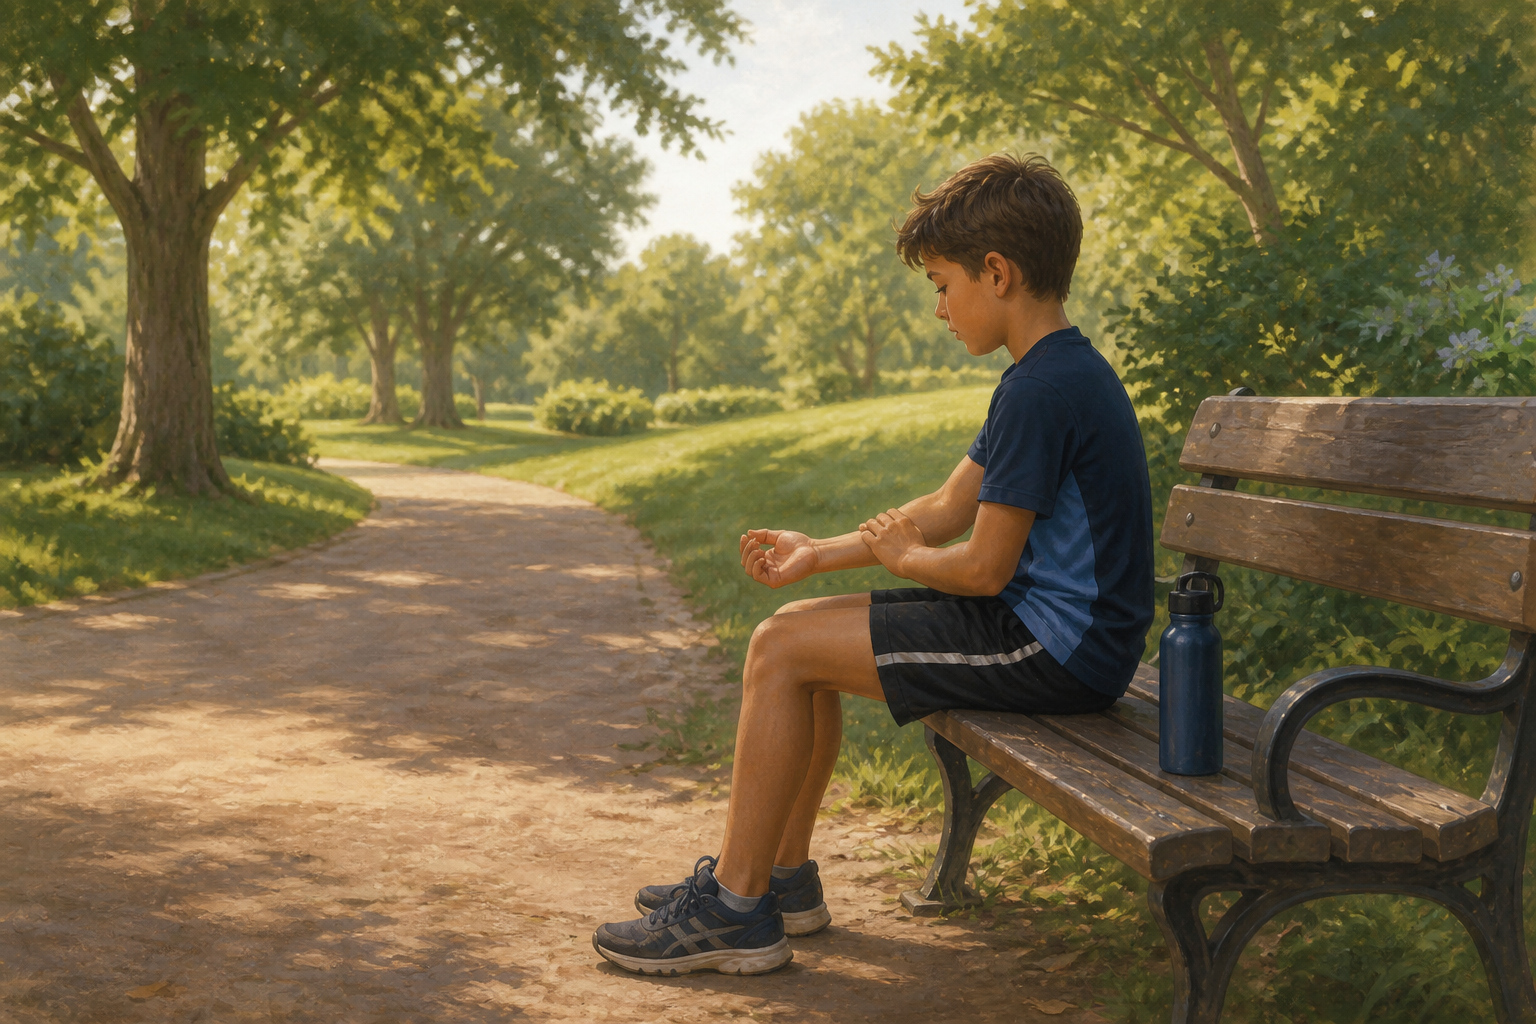
\includegraphics[width=0.58\linewidth]{images/book1/ai/g4-heart-rest.png}

{\small Después de la carrera: dos dedos en la \omterm{def:g1:my-body:joint}{muñeca}, contando desde
lejos la carrera del \omterm{def:g4:heart-and-blood:heart}{corazón}.}
\end{omfigure}

\begin{remark}[Un músculo que no descansa nunca --- casi]\label{rem:g4:heart-and-blood:rest}
Entre dos \omterm{def:g4:heart-and-blood:heart}{latidos} el \omterm{def:g4:heart-and-blood:heart}{corazón} se relaja una fracción de segundo --- ese
pellizco es todo el descanso que se toma. Día y noche, unos $100000$
\omterm{def:g4:heart-and-blood:heart}{latidos} al día, durante una vida entera. Como todos los \omterm{def:g3:bones-and-muscles:muscle}{músculos}
(\cref{met:g3:bones-and-muscles:care}), se hace más fuerte con el
ejercicio: un \omterm{def:g4:heart-and-blood:heart}{corazón} entrenado mueve más \omterm{prop:g4:journey-of-food:absorb}{sangre} en cada \omterm{def:g4:heart-and-blood:heart}{latido}, y por
eso puede latir con más calma.
\end{remark}

\section{Ejercicios}

\begin{exercise}[$\star$]\label{exo:g4:heart-and-blood:1}
Nombra dos cosas que reparte la \omterm{prop:g4:journey-of-food:absorb}{sangre} y dónde recoge cada una.
\end{exercise}

\begin{exercise}[$\star$]\label{exo:g4:heart-and-blood:2}
¿Qué gas de desecho se lleva la \omterm{prop:g4:journey-of-food:absorb}{sangre} y dónde lo deja?
\end{exercise}

\begin{exercise}[$\star$]\label{exo:g4:heart-and-blood:3}
¿De qué está hecho el \omterm{def:g4:heart-and-blood:heart}{corazón}, qué tamaño tiene y dónde está?
\end{exercise}

\begin{exercise}[$\star$]\label{exo:g4:heart-and-blood:4}
¿Qué hace cada lado del \omterm{def:g4:heart-and-blood:heart}{corazón}?
\end{exercise}

\begin{exercise}[$\star$]\label{exo:g4:heart-and-blood:5}
¿Qué es el \omterm{prop:g4:heart-and-blood:pulse}{pulso} y qué te dice contarlo?
\end{exercise}

\begin{exercise}[$\star$]\label{exo:g4:heart-and-blood:6}
¿Por qué hay que tomar el \omterm{prop:g4:heart-and-blood:pulse}{pulso} con los dedos y no con el pulgar?
\end{exercise}

\begin{exercise}[$\star$]\label{exo:g4:heart-and-blood:7}
¿Por qué se dispara el \omterm{prop:g4:heart-and-blood:pulse}{pulso} durante un esprint? Cuenta la historia
desde el punto de vista de los \omterm{def:g3:bones-and-muscles:muscle}{músculos} de las \omterm{def:g1:my-body:parts}{piernas}.
\end{exercise}

\begin{exercise}[$\star$]\label{exo:g4:heart-and-blood:8}
Pruébalo: tómate el \omterm{prop:g4:heart-and-blood:pulse}{pulso} en reposo con el
\cref{met:g4:heart-and-blood:pulse}, haz treinta segundos de saltos de
estrella y vuelve a tomártelo. Da los dos números.
\end{exercise}

\begin{exercise}[$\star\star$]\label{exo:g4:heart-and-blood:9}
En el \cref{ex:g4:heart-and-blood:round}, la gota de \omterm{prop:g4:journey-of-food:absorb}{sangre} sale roja
brillante de los \omterm{def:g4:breathing:organs}{pulmones} y más oscura del \omterm{def:g3:bones-and-muscles:muscle}{músculo} de la \omterm{def:g1:my-body:parts}{pierna}. ¿Qué
cambió en ella cada vez?
\end{exercise}

\begin{exercise}[$\star\star$]\label{exo:g4:heart-and-blood:10}
La \omterm{prop:g4:journey-of-food:absorb}{sangre} conecta tres órganos de tu curso: \omterm{def:g4:journey-of-food:tract}{intestino delgado},
\omterm{def:g4:breathing:organs}{pulmones} y \omterm{def:g4:heart-and-blood:heart}{corazón}. Dibuja o describe la red: ¿qué aporta cada uno al
servicio de reparto?
\end{exercise}

\begin{exercise}[$\star\star\star$]\label{exo:g4:heart-and-blood:11}
El \omterm{prop:g4:heart-and-blood:pulse}{pulso} en reposo de un ciclista entrenado puede ser de $50$; el de
un adulto sin entrenar, de $75$. Con la
\cref{rem:g4:heart-and-blood:rest}, explica cómo \emph{más lento}
puede significar \emph{más fuerte} --- ¿qué tiene que estar haciendo
cada \omterm{def:g4:heart-and-blood:heart}{latido} del ciclista?
\end{exercise}
